\section{Introducción}
En esta sección se hará una contextualización y se profundizará sobre qué es la generación procedural, realizando un análisis e investigación de aquellos antecedentes, técnicas, algoritmos e implementaciones previas, así como se analizarán otras herramientas que tengan que ver con la generación de mapas de manera procedural, tanto para Unity como para otro tipo de motores o plataformas, y se realizará una comparación entre estas y el trabajo realizado en este TFM.

Se investigará sobre los distintos algoritmos de generación de mapas de alturas, de biodiversidad, de teselación, de reducción de geometría para LOD, sobre el uso de Job System (tipos de Jobs y cuáles son más apropiados), modelos de distribución probabilística para instanciación de assets, técnicas de simulación de agentes y climas, de modelación en base a masas de agua, sobre métodos de optimización de la inmersividad y más.

\section{Contextualización}
    \subsection{Definición y Conceptos Básicos}
    
    La generación procedural o generación por procedimientos, también conocida como PTG (Procedural Content Generation) es una técnica que consiste en la creación de datos a través de algoritmos en tiempo real en lugar de generar estos datos de manera manual.
    
    Esta técnica se utiliza habitualmente en gráficos por computador, simulación y videojuegos. En el ámbito de la los gráficos se utiliza para la creación de texturas o geometría.
    
    En videojuegos se utiliza en compresión y reutilización de datos, escalabilidad o mejorar la rejugabilidad. Concretamente, en el ámbito de videojuegos la generación procedural se usa para generación de niveles para juegos estilo 'Rogue', generación de terrenos y mapas para juegos de mundo abierto, diálogos, instanciación de objetos, etc.\cite{procedural-generation-overview}.

    También se ha utilizado para otros diversos fines, como cine para el desarrollo de un gran número de objetos similares con pequeñas variaciones que dan lugar a staff decorativo y efectos visuales. Un ejemplo de sus uso en el cine es el Señor de los Anillos, donde se usó esta técnica para la generación masiva de soldados. \cite{generacion-procedimental-wikipedia}

    Las razones más comunes para el uso de la generación procedural incluyen: archivos de menor tamaño, mayor cantidad de contenido que se pueden crear manualmente o la inclusión de aleatoriedad para experiencias de juego más sorprendentes. \cite{generacion-procedimental-wikipedia}

    Cabe mencionar que a menudo se confunde el térmico generación aleatoria con generación procedural, que no son equivalente. La generación aleatoria está englobada en la generación procedural, pero carece guías ni restricciones, por lo que puede producir resultados indeseados y anárquicos. 

    Por último, para mencionar las ventajas y desventajas que supone esta técnica mencionaré algunos pros y contras:

    \begin{itemize}[label=--]
        \item \textbf{Pros:}
        \begin{itemize}[label=$\bullet$]
            \item Archivos de menor tamaño.
            \item Menor esfuerzo para agregar gran cantidad de contenido.
            \item Jugabilidad menos repetitiva, por tanto mejor rejugabilidad.
            \item Mayor eficiencia y resultados coherentes.
            \item Produce resultados reproducibles usando los mismos parámetros.
        \end{itemize}
        \item \textbf{Contras:}
        \begin{itemize}[label=$\bullet$]
            \item Más difícil visualizar y depurar los algoritmos durante su creación.
            \item Dificultad para cambiar el algoritmo una vez construido.
            \item Sin un conjunto definido de reglas, la generación procedural puede volverse muy desordenada y potencialmente romper el juego.
            \item Puede llevar más tiempo crear un algoritmo que la creación manual.
        \end{itemize}
    \end{itemize}

    \subsection{Historia y Evolución}
    La generación procedural de contenido para videojuegos se remonta al propio comienzo de la industria de los videojuegos. En la década de 1970, Don D. Worth utilizó algoritmos simples en su juego de Beneath Apple Manor para crear mazmorras en este RPG. Posteriormente, en 1980, se lanzó 'Rogue' que también era un juego de mazmorras con creación de niveles. Este juego, además, fue referencia para la generación posterior de juegos con las siguientes características:
    \begin{itemize}
        \item Jugabilidad por turnos.
        \item Niveles generados proceduralmente.
        \item Muerte permanente (sin funcionalidad de carga/guardado).
    \end{itemize}

    Que pasaron a llamarse juegos de tipo Rogue. \cite{ProceduralContentCreation}

   
    \begin{figure}[h]
        \centering
        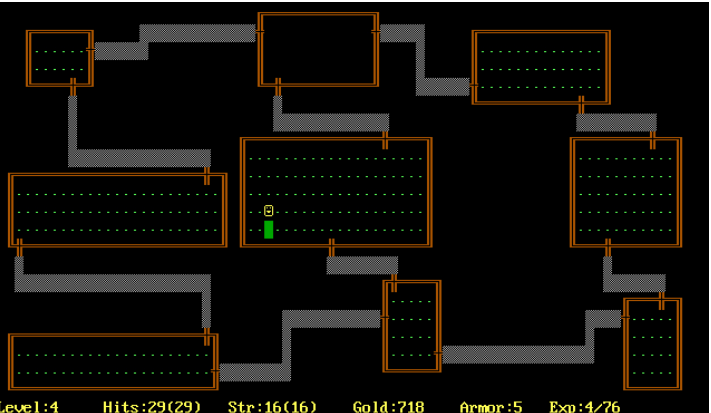
\includegraphics[width=0.5\textwidth]{img/Rogue.png}
        \caption{Mapa generado del videojuego Rogue primera versión ASCII.}
        \label{fig:1.0}
    \end{figure}
        
    

    Los primeros videojuegos gráficos fueron frenados por las fuertes limitaciones de memoria. Esto provocó que el contenido, como mapas, fuera generado algorítmicamente ya que simplemente no había espacio suficiente para almacenar una gran cantidad de niveles preconstruídos y arte de los niveles.
    
    Existen varios ejemplos de generación procedural en los primeros juegos. Por ejemplo, 'Akalabeth' (1980) de Richard Garriott utiliza semillas para generar el mundo, permitiendo a los jugadores regresar a un mundo dado utilizando el mismo número de semillas. Otro ejemplo fue 'The Sentinel', en el cual se almacenaron supuestamente diez mil niveles diferentes en solo unos pocos kilobytes. 'Elite', otro juego que hizo uso el PCG, originalmente planeaba tener un número masivo de galaxias, pero solo se seleccionaron ocho debido al temor de que un universo tan vasto resultara poco creíble para los jugadores. Otros ejemplos notables incluyen 'Rescue on Fractalus' (1985), que emplea fractales para crear montañas alienígenas, y 'River Raid' (1982) de Activision, que utiliza números pseudoaleatorios para generar obstáculos en un laberinto desplazable. \cite{generacion-procedimental-wikipedia}

    Ya en la década de los 90, el artículo 'Solid Texturing' de Darwin R. Peachey, publicado en 1985 \cite{Peachey1985}, fue una de las primeras publicaciones que trataba explícitamente sobre la generación de contenido procedural, donde se proponía una técnica similar al mapeo de normales actual para que las texturas bidimensionales pareciesen tridimensionales. De este artículo surgieron nuevas publicaciones que daba lugar a la generación procedural como campo de investigación dado que estos trataban sobre generación de terreno \cite{LeeUrban2016} o diseño de plantas mediante fractales \cite{Oppenheimer1986}.
    
    Un ejemplo de los resultados de iniciar la investigación en generación procedural fue la herramienta RenderMan, de Pixar, la cual servía para generar texturas, materiales y primitivas simples para usarlas en animación, por lo que la generación procedural transgredió los videojuegos y se empezó a usar en más ámbitos.

    Posteriormente en la década de los 2000 y con el aumento de la investigación, las técnicas para la generación mejoraron y se empezaron a usar en juegos AAA donde el PCG se usaba como un elemento concreto del juego, no por obligación debido a la falta de recursos como en épocas anteriores. Algunos juegos de estos años que usaron esta técnica fueron: Command and Conquer: 'Red Alert 2' (2000), 'Diablo' (1996) y 'The Elder Scrolls II: Daggerfall'. \cite{ProceduralContentCreation}

    En 2004, el grupo '.theprodukkt' lanzó un shooter llamado '.kkrieger'. Este juego, que ganó el primer lugar en la competencia de juegos de 96k en Breakpoint en abril de 2004 no llegó a ser lanzado, permaneció como una demo. El objetivo de este juego fue demostrar la capacidad de generar un videojuego con un tamaño extremadamente reducido, generando texturas, modelos, animaciones, música y niveles usando con herramientas procedurales. Los desarrolladores decidieron publicar sus herramientas en forma del editor .werkkzeug. \cite{WikipediaKkrieger}
    
    \begin{figure}[h]
        \centering
        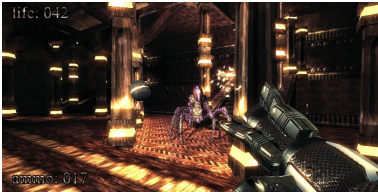
\includegraphics[width=0.5\textwidth]{img/.kkrieger.png}
        \caption{Muestra del juego .kkrieger. Tamaño del archivo: 96 kb}
    \end{figure}

    Como hemos visto, a comienzos del nuevo milenio, el almacenamiento dejó de ser un problema y la creación de escenarios se volvió más sencilla, en gran parte gracias a los nuevos motores gráficos como Unreal Engine 4 o Unity3D. Esto, junto con la disminución de la popularidad del género Roguelike, frenó el progreso de los métodos de generación procedural.

    Sin embargo, el lanzamiento de 'Minecraft' en 2011 cambió esto completamente, ya que su popularidad volvió a destacar la generación procedural y su otra gran virtud, la variedad de contenido y rejugabilidad. En Minecraft, cada partida crea un mundo completamente diferente al anterior, lo que permite a los jugadores volver a jugar el juego y experimentar nuevas experiencias.
    
    Minecraft supuso un punto de inflexión para la generación procedural en los videojuegos, siguiendo aún vigente a día de hoy, demostrando que los juegos basados en rejugabilidad, mundo abierto y generación procedural con elementos cambiantes y dinámicos están más viva que nunca.

\section{Antecedentes}

    La generación procedural de contenido ha sido fundamental en el desarrollo de entornos virtuales y videojuegos, permitiendo la creación dinámica de terrenos, biomas, ciudades y otros elementos de manera eficiente y escalable. En este apartado, se examinarán las herramientas y trabajos previos relacionados con la generación procedural, centrándose principalmente en las aplicaciones para motores gráficos como Unity y Unreal Engine.

    \subsection{Herramientas para Unity y Otros Motores}

    Para crear terrenos en Unity existen diversos assets, disponibles tanto como asset del asset store como softwares independientes. Aquí una lista con descripciones de algunos de los softwares más utilizados en la actualidad categorizados por sus funcionalidades y propósito:

        \subsubsection{Generación de Terrenos y Paisajes} 
            \begin{itemize}[label=\textbullet]
                \item \textbf{Terrain Generator: }   
                Esta herramienta de la asset store de Unity permite la generación paramétrica de terrenos complejos mediante cálculo masivo en GPU, los cuales se pueden modificar mediante un sistema de nodos pudiendo añadir simulaciones físicas realistas. También cuenta con un sistema de generación de biomas, pudiendo mezclar biomas ya generados. Actualmente es un asset de pago con dos ediciones: Indie y Pro. \cite{unity-assetstore-terrain-generator-vista-pro}

                \item \textbf{MapMagic:} 
                Herramienta diseñada para Unity de pago que se puede integrar importándolo en el propio Unity. Es un generador de mapas basado en nodos que cuenta con módulos adicionales que permiten colocar objetos y generar biomas y caminos. Los nodos de esta herramienta representan generadores de terreno (ruido, voronoi, etc.) u objetos (mezcla, curva, erosión, etc.) cuya acción conjunta permite crear los terrenos. Además, existe una paquete adicional: MapMagic2 que cuenta con módulos adicionales que añade más funciones. Además de ser integrable con Unity, si se desea integrar en el workflow con otros motores se pueden exportar los terrenos generados para ser usados en estos adaptando los datos a los formatos específicos de cada motor. \cite{unity-assetstore-mapmagic-world-generator}
                
                \item \textbf{Terrain Composer 2: }
                Terrain Composer 2 es otra herramienta del asset store de Unity que consiste en un generador de 'tiles' de terreno basado en nodos mediante GPU que utiliza un sistema basado en capas.

                Algunas otras características destacables son la exportación de mapas de altura, de texturas, color y normales; su integración con RTPv3 ("Relief Terrain Pack Version 3", un conjunto de herramientas para Unity que proporciona una serie de shaders y funciones avanzadas para crear terrenos realistas), biblioteca completa de ruido, incluyendo ruidos erosionados, entre otras. Esta herramienta también es de pago pero con un precio menor que las anteriores. \cite{unity-assetstore-terrain-composer-2}
                
                \item \textbf{Terragen: }
                Terragen es un software utilizado para construir, renderizar y animar entornos naturales realistas, mediante la importación de da6tos de alturas o mediante el uso de un editor de terreno con funciones procedurales integradas para lograr terrenos a escala global con un grado detalles enorme. Este software permite tener control, además de sobre el terreno, sobre el clima, ríos, lagos, océanos, etc. y también ofrece control de los shades utilizados para terrenos, texturas, desplazamientos de micropolígonos, nubes y distribución de objetos con formato nativo TGO u OBJ que pueden haber sido modelados en otros softwares. 

                Otras características reseñables de esta herramienta es que posee un renderizador híbrido de micropolígonos y trazado de rayos, especialmente optimizado para manejar grandes desplazamientos y paisajes de gran escala. Un sistema de iluminación global a 'escala planetaria' para simulación de sistemas planetarios. Una atmósfera fotorrealista con control sobre las nubes con efectos volumétricos y '2.5D'. Opciones de animación de parámetros y editor de nodos para control de texturas y sombreados. Por último es integrable con otros motores mediante la exportación de sus modelos en alta resolución. \cite{TerragenOverview}
                
                \item \textbf{Gaia:}
                Este asset de pago de la asset store de Unity permite generar terrenos y paisajes para móviles, realidad virtual, consolas y escritorio tanto fotorrealistas como lowpoly. Cuenta con un sistema de edición de terrenos permitiendo un workflow artístico y procedural en la generación de paisajes. También cuenta con un sistema de generación de biomas, aldeas y de configuración de viento, agua y efectos, incluyendo efectos de sonido para dar una mayores sensación de inmersión. Múltiples sistemas de cielo e iluminación (incluido el momento del día), sistema meteorológico con soporte para lluvia y nieve, sistema de agua y shaders de alto rendimiento. Es un software acelerado por GPU con tiene soporte integrado con URP y HDRP.

                Otra característica muy destacable de este asset es el conjunto de assets de muestra con los que viene, el cual se puede personalizar añadiendo o quitando assets de esta colección pudiendo generar los diferentes biomas en base a estos assets. Además, cuenta con una versión pro que añade aún más funcionalidades y activos. \cite{unity-assetstore-terrain-generator-vista-pro} \cite{GaiaPro}
                
                \item \textbf{Gaea: }
                Gaea es un software independiente especializado en la generación procedural de terrenos y paisajes, incluyendo formas geológicas, simulaciones de erosión, nieve y ríos, herramientas para edición de rocas y generador de texturas basado en nodos. Este software posee un sistema basado en nodos para realizar simulaciones. Esta herramienta presenta un flujo de trabajo no destructivo, lo que permite iterar sobre los paisajes para actualizar los terrenos generados. Con este software se pueden crear formas de manera procedural utilizando primitivas e importar modelos texturizados y convertirlos en terrenos. Una característica destacable de este software es su algoritmos de erosión, el cual posee flexibilidad para brindar control artísticos sobre la apariencia. Además de los terrenos también están sus biomas, pudiendo recrear ecosistemas complejos con datos relevantes como zonas en conflicto, nieve, agua y más. 

                Este software permite también la creación de texturas sofisticadas utilizando mapas de datos, además de la personalización de los mismos junto con la exportación de máscaras, incluidos mapas PBR para poder texturizar en otros motores. Los terrenos generados en este motor son exportables con alta calidad gracias a su soporte para formatos universales junto a su generación de LOD automáticos. \cite{QuadSpinner}

                \item \textbf{World Creator:}
                World Generator es otro software independiente de esta lista para generación de terreno procedural. Este software permite generar terrenos haciendo uso de cálculo en GPU de cualquier tamaño con  diferentes grados de detalle. Además, posee herramientas de edición y escultura del terreno pudiendo no solo modificar su forma sino su mapa de colores. También permite crear ríos, montañas, carreteras y demás accidentes geográficos, así como efectos de erosión realista, entre otras características. Al igual que las demás herramientas anteriores, también permite la generación de biomas y cuenta con una gran librería de ellos predefinida. 
                
                Este software cuenta con us propio motor de render con Ray-tracer en GPU. Además, es compatible universalmente, por lo que los terrenos generados en este software se pueden integrar con otros motores como Unity, Unreal Engine, Blender, etc. mediante la exportación de los terrenos generados en diversos formatos. Este software profesional de pago cuenta con su propia documentación y tutoriales, lo que lo hace muy completo. \cite{world-creator-website}
                
                \item \textbf{World Machine:}
                World Machine es otro software independiente que permite la creación de terrenos con diferentes aspectos, desde realistas hasta terrenos estilizados, ello posible gracias a su generación basada en fractales mediante un workflow de nodos que permite la edición del mismo con herramientas propias. También cuenta con sistemas de agua para crear efectos geológicos realistas, ríos, lagos, etc.; sistema de texturizado de materiales con soporte para renderizado basado en física (PBR) y exportación de terrenos como mapas de altura, malla y los datos de materiales, los cuales se pueden exportar en una variedad de formatos. También se pueden exportar escenas completas con GLTF.

                Este software, también profesional de pago posee diversas funcionalidades y utilidades para la generación de terrenos  con compatibilidad con motores como Unity y Unreal Engine, o renderizadores 3D como Blender, Maya o Cinema4D. \cite{world-machine}

                \item \textbf{Vue:}
                Este software es un paquete de entornos profesional que cuenta con varios tipos de licencia: Creator, Professional y Enterprise, utilizado para la creación de entornos y paisajes. Cuenta con herramientas para artistas para la generación procedural de vegetación y terrenos, pudiendo crear incluso planetas. A través sus herramientas de pintura manual de los terrenos, se puede lograr un mayor control sobre la apariencia final del terreno, que en combinación con ruidos y fractales procedurales da lugar a resultados realistas. Además, VUE cuenta con un modelo atmosférico que simula condiciones de iluminación realistas. VUE además proporciona una gran biblioteca de assets de plantas para crear escenas de vegetación variadas. Este software se puede integrar con motores como Unity o Unreal mediante plugins y permite la exportación de sus escenas o activos en una amplia variedad de formatos. \cite{VUEOverview} 
            \end{itemize}

        \subsubsection{Herramientas Procedurales Generalistas}

            \begin{itemize}[label=\textbullet]

                \item \textbf{Houdini:}
                Houdini es uno de los softwares más famosos en la industria de los VFX dada su increíble versatilidad ya que se puede utilizar para producir prácticamente de todo, y los terrenos no son una excepción. Si bien no es un software específico para este fin, la versatilidad que posee permite dar lugar a terrenos generados algorítmicamente, físicamente realistas, editables y exportables. En Houdini los terrenos se pueden generar utilizando varios métodos, pero el más común es el uso de nodos y operadores procedurales que combina la generación de ruidos con operaciones matemáticas que esculpen el terreno. El terreno se puede generar mediante la combinación de fractales de terreno junto con el uso de máscaras para lograr efectos detallados y realistas, produciendo fracturas, erosiones, texturas mediante capas de ruido y nodos de deformación. Además, Houdini cuenta con herramientas de escultura para personalizar los terrenos generados y se pueden repartir assets con la distribución de objetos mediante nodos procedurales.
                
                Houdini es una herramienta de tal magnitud, que a pesar de no ser específica para generar este tipo de assets permite la producción de terrenos totalmente personalizables y con alto grado de realismo, con capacidad de exportación a otros softwares como Unreal. Si bien es un software generalista que no permite la generación en tiempo real, al igual que los otros softwares independientes, merece estar en esta lista. \cite{sidefx} \cite{creativebloq}
            \end{itemize}

        \subsubsection{Herramientas de Generación de Entornos Urbanos}
        
            \begin{itemize}[label=\textbullet]
                \item \textbf{EasyRoads3D: }
                EasyRoads es un asset gratuito disponible en la asset store de Unity, cuya función es la generación de carreteras de manera eficiente en Unity. Si bien no se puede decir que EasyRoads sea una herramienta procedural, pues la creación de carretas se realiza de manera manual, es un asset muy utilizado para la creación de entornos en terrenos que sí han podido ser generados proceduralmente de manera rápida y que en combinación con scripts propios, sí puede ser usado de manera automatizada. Es por esto que ha sido incluida en esta lista, aunque sea como mención complementaria. \cite{easyroads3d}
                
                \item \textbf{CityGen3D:}
                CityGen3D es otro asset de pago de la tienda de Unity utilizado para la generación de ciudades a partir de datos sobre carreteras, árboles, edificios, etc. utilizando información de OpenStreetMas. Esta herramienta permite la importación de mapas de altura del terreno, generación automática de carreteras, edificios procedurales con niveles automáticos de detalle (LOD), generación de biomas. Otras características de este asset es su compatibilidad con diferentes render pipelines de Unity, como el High Definition Render Pipeline (HDRP), Universal Render Pipeline (URP) y el Built-In pipeline, lo que la hace aún más completo. \cite{CityGen3DUnityAssetStore} \cite{CityGen3DWebsite}
                
                \item \textbf{Building Generator:}
                Este asset de bajo costo en la tienda Unity es un generador de edificios como su propio nombre indica que permite construir y pintar edificios utilizando parte premodeladas que ensambla y asigna materiales seleccionados generando una malla única combinada. \cite{BuildingGenerator}

                No es una herramienta procedural en sí al igual que pasaba con otras anteriores pero que puede jugar un papel muy útil en la generación de ciudades para mapas procedurales, sumado a los mecanismos procedurales en su funcionamiento que parece tener, se ha incluido en esta lista.
                
                \item \textbf{CityEngine: }
                CityEngine es un software de modelado 3D avanzado para crear entornos urbanos enormes, interactivos e inmersivos en menos tiempo que las técnicas de modelado tradicionales. Las ciudades que crees utilizando CityEngine pueden basarse en datos SIG del mundo real o mostrar una ciudad ficticia del pasado, presente o futuro. Este software permite crear ciudades en 3D y diseñar entornos urbanos creando modelos gracias a sus herramientas de edición. Permite traer activos para construir un contexto 3D alrededor y exportar el trabajo para llevarlo de nuevo a un software de visualización o motor como Unity o Unreal. Además, permite automatizar los flujos de trabajo con código procedural y Python. \cite{EsriCityEngine} 
            \end{itemize}

        \subsubsection{Herramientas de Generación de Vegetación}

            \begin{itemize}[label=\textbullet]

                \item \textbf{Vegetation Studio Pro: }
                Este también es un asset gratuito de la tienda de Unity añade funcionalidades a su versión anterior (Vegetation Studio). Este software, al igual que EasyRoads3D suele usarse sobre terrenos ya generados para agilizar y realizar la población del terreno con vegetación de manera eficiente. Algunas de las características de esta herramienta son la creación de máscaras de biomas, funciones por lotes para ajustar configuraciones de biomas, y la creación de áreas de máscara para la vegetación, entre otras. 

                Aunque no es una herramienta procedural en sí misma, es una herramienta que se integra con la generación de terrenos procedurales permitiendo la creación y manejo de biomas, por lo que es una herramienta habitual a la hora de generar paisajes con biomas, tema sobre el que trata el trabajo de este proyecto \cite{UnityAssetStoreVegetationStudioPro}. Al igual que no el asset anterior, esta son las razones para incluirla en esta lista.
                
                \item \textbf{SpeedTree:}
                SpeedTree es un software independiente profesional de pago con integración en Unity. Esta herramienta se utiliza para el modelado de vegetación permitiendo la creación vegetación realista de forma rápida y eficiente, por lo que es un asset valorado por su uso en la generación de biomas escenarios naturales. Esta herramienta ofrece capacidades de modelado manual pero también de generación procedural, permitiendo a los usuarios crear variaciones de la vegetación con control sobre parámetros específicos. Algunas de las características de la herramienta en las que se emplean técnicas procedurales son procedurales: randomización, colisión de hojas,  Mesh anchors, Clusters, Divisiones de la mesh, Control de la forma, color de los vértices, manipulación de secciones de la mesh, UV tiling, entre otras. \cite{UnitySpeedTree}
            \end{itemize}

        % \subsubsection{Herramientas de Simulacion Climática}
        %     \begin{itemize}[label=\textbullet]
        %         \item \textbf{Enviro: }
        %         Este asset de pago (bajo precio) de la tienda de Unity es una herramienta que ofrece un sistema meteorológico para Unity que permite crear y controlar clima, iluminación, cielo, niebla y nubes. Es un asset utilizado para la creación de efectos climáticos en combinación con sistemas de partículas como tormentas eléctricas, nieve y niebla. El asset viene con un paquete de climas predefinidos como: Cielo despejado, Nublado, Lluvioso, Tormentoso, Nevado y Brumoso. Además, también incluye ciclos de noche y día sincronizando la hora del sistema, shaders de skybox atmosféricos configurable. \cite{GameAssetDealsEnviro} \cite{UnityAssets4FreeEnviro3}

        %         Además de las funcionalidades mencionadas, posee diversas características como la integración con los sistemas de renderizado de Unity, soporte para RV, networking, y exportación de cubemaps HDR, entre otras. Aunque Enviro no es una herramienta de generación procedural en sí misma, es un recurso para creación de entornos procedurales al igual que EasyRoads3D o Vegetation Studio Pro dada su capacidad para simular fenómenos climáticos y crear entornos inmersivos y realistas habitual en entornos generados proceduralmente. \cite{UnityAssetStoreEnviroSkyWeather}

        %         \item \textbf{Tenkoku  :} ofrece cielo y clima de alta fidelidad completamente dinámicos, además de brindar la capacidad de simular el clima, el ciclo diurno y nocturno y las nubes. 
        %         \item \textbf{Massive Clouds Atmos  :}brinda la capacidad de representar todo el cielo con efectos volumétricos mientras lo ajusta para diversas condiciones climáticas. 
        %         \item \textbf{Expanse  :}una herramienta volumétrica de última generación para HDRP que le brinda el poder de crear hermosos cielos, nubes y bancos de niebla. 
        %         \item \textbf{Crest Ocean URP/HDRP  :} un sistema oceánico técnicamente avanzado y rico en funciones dirigido a plataformas de PC y consolas. 
        %         \item \textbf{KWS Water System Standard/URP/HDRP  :} un componente basado en módulos que le permite simular superficies de agua como un océano/mar/río/lago/piscina/etc. Sistema de agua dirigido a plataformas PC/consola y renderizado estándar. 
        %     \end{itemize}

    \subsection{Comparativa Entre las Distintas Herramientas y Este Trabajo}

    En el apartado anterior se han mostrado diferentes herramientas y assets, algunos de ellos únicos de la asset store de Unity, otros independientes con capacidad de exportar sus activos o con compatibilidad mediante plugins, y otros que poseen integración con alguno de los motores aunque se pueden usar de manera independiente también. Hay softwares que permiten la generación de terreno junto con biomas y/o aldeas, incluso fenómenos climáticos, otros a parte de la generación de terreno tienen compatibilidad con realidad virtual, otros son herramientas que permiten la modelación de los paisajes generados de manera automática o automatizable, que generan fenómenos atmosféricos y climáticos para construir escenas realistas, etc. 

    Todas las herramientas mencionadas cumplen con propósitos que se pretenden llevar a cabo en el proyecto de este TFM, pero la propuesta de este trabajo reúne características de estos softwares para crear una herramienta diferente, capaz de generar terrenos realistas, no en una fase de preprocesado para generar la escena, sino en el propio tiempo de ejecución, mientras el jugador se mueve, aprovechando al máximo la capacidad de cómputo de la CPU haciendo uso del sistema DOTS como principal innovación de esta propuesta. Además de este factor diferencial, en este proyecto no sólo se crearán terrenos en tiempo real con una tasa de refresco que permita una buena jugabilidad, sino que se generarán biomas, se hará distribución de assets correspondientes a la vegetación y demás elementos geográficos y se generaran asentamientos y poblaciones para dar un resultado más realista. Todo ello acompañado de compatibilidad con realidad virtual, efectos de sonido, fenómenos climáticos y edición del propio terreno generado. Este conjunto de funcionalidades, permiten suplir las diferencias de calidad con los resultados de aquellos que permiten una generación más detallada y realistas desde el punto de vista físico, así como de todos aquellos que mejoran los resultados producidos por la herramienta que se propone, pero no permiten que se utilice en tiempo de ejection, de manera procedural y con compatibilidad con realidad virtual dadas las experiencias que permite desarrollar en tiempo de ejecución. 

    Todas estas características de la solución que se proponen, añadido a que es un proyecto que pretende mejorar la calidad de los desarrollos de estudios con poca capacidad económica o indie teniendo un bajo precio o directamente la gratuidad en un hipotéticos caso de que saliera al mercado, hacen de esta herramienta un producto diferente y relevante dentro del mercado de herramientas y softwares destinados a la generación de terrenos, entornos y paisajes. 

    Los pros y contras de esta propuesta podrían resumirse de la siguiente manera:
    \begin{itemize}[label=--]
        \item \textbf{Pros:}
        \begin{itemize}[label=$\bullet$]
            \item Generación procedural de terrenos, biomas y elementos de entorno de buena calidad que mejoran la rejugabilidad.
            \item Integración Realidad Virtual para experiencias inmersivas.
            \item Más asequible que algunas herramientas comerciales.
        \end{itemize}
        \item \textbf{Contras:}
        \begin{itemize}[label=$\bullet$]
            \item Dada la cantidad de funcionalidades que integra la curva de aprendizaje puede ser elevada.
            \item Limitación en la calidad de los resultados dada la generación en tiempo real.
            \item Se requerirá de equipos con prestaciones mínimas para que sean capaces de producir resultados destacables con buena tasa de refresco.
        \end{itemize}
    \end{itemize}


    \section{Algoritmos y Técnicas más Utilizados y Aplicaciones}
    EbDavid S. Ebert identifica las siguientes características que deben estar presentes de las técnicas de generación procedural en su artículo "Texturing and Modelling - A Procedural Approach. Morgan Kaufmann. 2003" \cite{Ebert2003}
    \begin{itemize}
        \item \textbf{Abstracción:} Lo algoritmos deben generar resultados centrándose en el propósito general y dar resultados completo y no centrarse en los detalles.
        \item \textbf{Control Paramétrico:} Los parámetros se definen para que correspondan con un comportamiento específico.
        \item \textbf{Flexibilidad:} Para imitar la esencia de algo del mundo real, no es necesario una recreación totalmente explícita, lo que permite mayor flexibilidad en su implementación.
    \end{itemize}

    
    \subsection{Generación de Terreno}
       
        En este apartado se analizarán las técnicas y métodos más utilizados para generar mapas de alturas siguiendo la clasificación que se hace en \cite{Valencia-Rosado2019} y se nombrarán algunos nuevos métodos siguiendo técnicas más novedosas.

        La clasificación de técnicas generativas que se utilizan es la siguiente:

        \subsubsection{Métodos Estocásticos}
        Estos métodos, basados en el uso de parámetros, intentan generar resultados aleatorios, los cuales se pueden aplicar recursivamente para incrementar el detalle. Estos métodos se caracterizan por su rapidez y eficiencia -una de las razones principales por las que se ha decidido emplear esta técnica en este proyecto-. Aunque estos métodos son rápidos, no se pueden controlar la posición de las características de los terrenos generados (cañones, valles, etc.), que se generarán en posiciones aleatorias.
            \begin{itemize}
            \item \textbf{Fractales:}
            Estos métodos consisten en generar figuras autosemejantes mediante métodos iterativos o recursivos. Dentro de esta categoría quedan incluidos tanto los fractales caóticos como los ruidos para generar mapas de alturas. Algoritmos como:
                \begin{itemize}
                    \item \textbf{Ruido Perlin y Simplex:} El ruido Perlin es un tipo de ruido suave y continuo basado en la generación de valores pseudo-aleatorios desarrollado por Ken Perlin en la década de 1980. El ruido Simplex es una variación de este también desarrollado por Perlin en 2001, el cual genera mejores resultados visuales y en menor tiempo. Ambos métodos se pueden aplicar en varias capas con diferentes valores de frecuencia para generar un mapa de alturas fractal con detalles en diferentes escalas. \cite{PerlinNoise}
                    \begin{figure}[t]
                        \centering
                        \begin{minipage}[t]{0.7\textwidth}
                            \centering
                            \begin{minipage}[t]{0.45\linewidth}
                                \centering
                                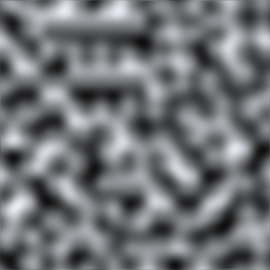
\includegraphics[width=\linewidth]{img/perlin-simple.png}
                                \caption{Ruido de Perlin simple.}
                                \label{fig:imagen1}
                            \end{minipage}\hfill
                            \begin{minipage}[t]{0.45\linewidth}
                                \centering
                                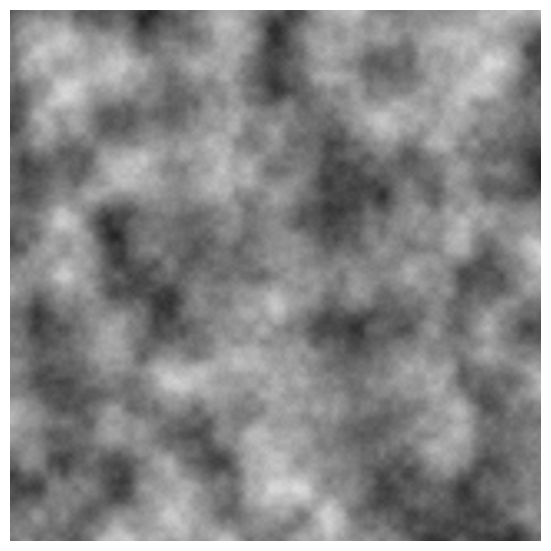
\includegraphics[width=\linewidth]{img/perlin-fractal.png}
                                \caption{Ruido de Perlin fractal.}
                                \label{fig:imagen2}
                            \end{minipage}
                        \end{minipage}
                    \end{figure}

                    \item \textbf{Ruido Worley:} El ruido de Worley es otro tipo de ruido que se genera en base a los diagramas de Voronoi, el cual produce patrones con estructuras celular que se genera dividiendo el espacio en celdas basadas en la distancia a un conjunto de puntos. A menudo se utiliza para generar terrenos con características como cuevas, crestas o túneles. \cite{worley-noise}
                    \begin{figure}[h]
                        \centering
                        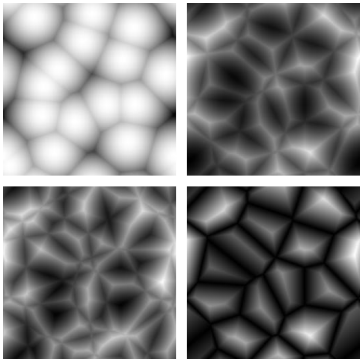
\includegraphics[width=0.5\textwidth]{img/voronoi-diagrams.png}
                        \caption{Ejemplos de diagramas de Voronoi con coeficientes $c_1 = -1$ (arriba izq.), $c_2 = 1$ (arriba der.), $c_3 = 1$ (abajo izq.), $c_1 = -1$ y $c_2 = 1$ (abajo der.).}
                        \label{fig:voronoi}
                    \end{figure}

                    \item \textbf{Algoritmo de desplazamiento del punto medio:} En este método se genera terreno fractal a partir de un segmentos y, en cada iteración, dividir cada segmento en dos partes. La altura de los nuevos vértices se ajusta mediante un valor de desplazamiento aleatorio inversamente proporcional al nivel de recursividad en el que se esté aplicando el desplazamiento, creando así características fractales. \cite{DesplazamientoPuntoMedio}
                    \item \textbf{Algoritmo diamante-cuadrado:} El algoritmo diamante-cuadrado consiste en dividir un cuadrado inicial con valores aleatorios en las esquinas en subcuadrados , donde la altura de los nuevos vértices se ajusta en función del promedio de los vértices originales. Este proceso se repite varias veces, lo que da como resultado un terreno con una apariencia fractal. \cite{DiamanteCuadrado}
                    \begin{figure}[h]
                        \centering
                        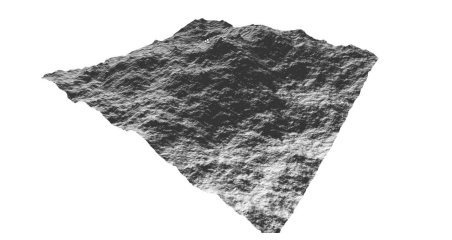
\includegraphics[width=0.7\textwidth]{img/terreno fractal.png}
                        \caption{Terreno generado con el algoritmo de desplazamiento del punto medio}
                    \end{figure}
                \end{itemize}

            \item \textbf{Gramáticas:} 
            Las gramáticas son reglas para la creación de lenguajes formales en los cuales secuencias en crecimiento se aplican a un estado inicial, en \cite{Marak_97} estas reglas se utilizan para deformar terrenos y así imitar las acciones de la erosión.
            Un ejemplo de método que utiliza las gramáticas son los L-Systems, los cuales se utilizan para generar fractales generando patrones a partir de reglas simples. Los Sistemas L fueron introducidos y desarrollados en 1968 por el biólogo y botánico teórico húngaro Aristid Lindenmayerc.
                \begin{figure}[h]
                    \centering
                    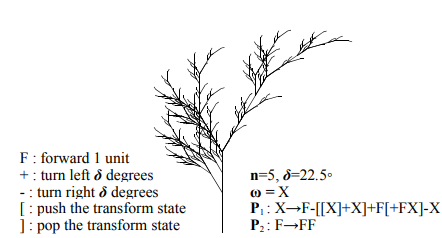
\includegraphics[width=0.6\textwidth]{img/L-systems.png}
                    \caption{Formación de árboles a través de un intérprete de sistemas-L.}
                \end{figure}

            \item \textbf{Tiling:} 
            Esta técnica consiste en dividir el terreno en áreas de menor tamaño. Una de estas técnicas y la más conocida son los Diagramas de Voronoi, los cuales dividen la superficie del terreno en superficies con forma celular.
            
            Con esta técnica se permite usar diferentes parámetros para cada división -o celda en caso de los diagramas de Voronoi- de manera que se pueda romper la regularidad producida por algoritmos como los basados en ruido produciendo transiciones entre distintas áreas más naturales.

            Tiling solo permite la división del terreno, por lo que es común que se utilice junto a otros algoritmos para la generación de terrenos como en el método descrito en \cite{olsen2004realtime}
            
            \item \textbf{Parametrización:} Estas técnicas giran en torno a tener instrucciones de construcción que son controladas por el usuario, quien ajusta sus parámetros. La variabilidad de los resultados está limitada por el número de parámetros controlables. En \cite{Choros2016} se presenta un método basado en la parametrización de tiles. En \cite{Yin2013} se propone un método para crear cordilleras, los parámetros son altitud, pendiente y área de influencia.
            
            \end{itemize}

        \subsubsection{Métodos de Simulación}
        Los métodos de simulación física pueden utilizarse en la generación procedural de terrenos para crear terrenos más realistas emulando fenómenos naturales y efectos de procesos físicos como la erosión, la deposición y la meteorización en el terreno, lo que da como resultado un terreno más realista. Algunos de los algoritmos de los métodos simulación más comunes son:

            \begin{itemize}
                \item \textbf{Geomorfológicos:}  
                La erosión es uno de los principales factores de la formación del terreno, y estos enfoques se centran en la simulación de formas realistas. Suelen emplearse posteriormente a otros métodos de generación -como los métodos fractales- para añadir una capa de realismo. 
                
                Dentro de esta categoría se pueden incluir los siguientes métodos:
                \begin{itemize}
                    \item \textbf{Basados en hidrología}: Los algoritmos basados en hidrología simulan el flujo del agua sobre el terreno, teniendo en cuenta factores como la pendiente, la lluvia y la evaporación. Estos algoritmos pueden utilizarse para crear terrenos con redes de ríos realistas, lagos y otras características de agua \cite{AlgoritmosHidrologia} \cite{HidrologiaDocumento}. En \cite{Fischer2022} se describe un modelo de generación de terrenos a partir de las masas de agua del mismo.
                    \item \textbf{Basados en erosión}:  Dentro de los algoritmos de erosión existen dos principales: la erosión térmica y la hídrica, en los cuales se simulan los efectos de la erosión causada por el agua, el viento en el terreno o el desprendimiento de partes de terreno dado un ángulo de inclinación o talud, lo que da como resultado terrenos con características como valles, crestas y cañones. Como se ha mencionado anteriormente, estos suelen utilizarse en conjunto con otras técnicas como funciones de ruido o fractales. \cite{AlgoritmosErosion} \cite{ErosionReddit}. Esta técnica se  puede observar también en  \cite{olsen2004realtime}. 
                    \item \textbf{Choque de placas tectónicas:} El levantamiento de terreno debido a la simulación de choques entre placas tectónicas también entra en esta categoría. Este proceso eleva todo el terreno con el tiempo provocando la creación de sierras. En \cite{Cordonnier2016} se emplea este método para para simular los procesos tectónicos que dan forma al terreno a gran escala y la deformación del terreno generando elevaciones y depresiones.
                    
                \end{itemize}
        
                \item \textbf{Ecosistemas:}
                Los métodos basados en ecosistemas, también llamados biomas, alteran la apariencia del terreno provocando que por ejemplo, dos terrenos con la misma apariencia geomorfológica luzcan de manera totalmente distinta debido a la presencia de vegetación u otros elementos ambientales que definan ecosistemas distintos. 

                La simulación de ecosistemas para modelar la apariencia del terreno a menudo se lleva a cabo mediante sistemas multicapa como en \cite{autobiomes}, donde se genera el terreno siguiendo un pipeline de varias capas calculando en ellas factores como la humedad, temperatura y el viento para simular las condiciones del terreno. En \cite{Cordonnier2017} se realiza un proceso similar, donde en función de la humedad y exposición al sol se genera vegetación.

                Algunas de los métodos más empelados son:

                \begin{itemize}
                    \item \textbf{Modelos Hidrológicos} Son modelos que simulan la influencia de masas de agua  y las cuencas hidrográficas para la distribución de los diversos biomas junto con efectos adicionales como la erosión. El artículo \cite{Fischer2022}, en su método describe también la distribución de biomas basada en cuerpos de agua durante la generación.
                    \item \textbf{Diagrama de Voronoi}: Este enfoque permite la generación de terrenos con diversos biomas basándose en los diagramas de Voronoi para su distribución. En el paper \cite{olsen2004realtime} se emplea este método.
                    \item \textbf{Reglas Geográficas}: Este método emplea reglas y parámetros como la latitud para asignar biomas de manera realista. En el método propuesto en \cite{Choros2016}, además de emplear diagramas de Voronoi, tiene en cuenta la latitud para controlar el tipo de biomas generados. 
                    \item \textbf{Distribución de Altura:} Este enfoque simula biomas con diversidad en función de la altitud de los terrenos generados. En el paper de Jacob Olsen \cite{olsen2004realtime} de nuevo, se emplea este método para generar diversidad en los biomas.
                    \item \textbf{EDPCG (Experience-Driven Procedural Content Generation):} En \cite{AnalisisAlgoritmosAmbientesVirtuales} se describe el algoritmo EDPCG, el cual se emplea para ajustar los modelos generativos en base a la experiencia del usuario. Aunque no es un algoritmo o método estrictamente circunscrito a la generación de biomas específicamente en el artículo se nombra como método para la generación de contenido, lo que puede incluir la instanciación de assets o elementos, lo cual está íntimamente relacionado con el modelado de biomas, y puede ser un método a considerar en esta clasificación.
                \end{itemize}

                \begin{figure}[h]
                    \centering
                    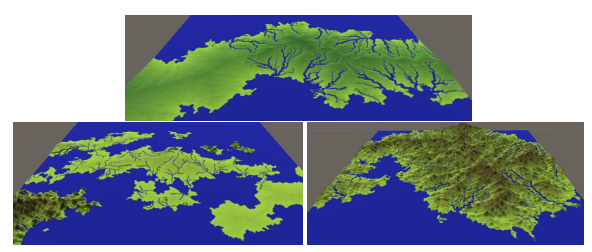
\includegraphics[width=0.8\textwidth]{img/procedural landscape with watrerbodies.png}
                    \caption{Terreno generado basado en cuerpos de agua \cite{Fischer2022}}
                \end{figure}
                
                \item \textbf{Basados en Agentes:} Estos métodos no se basan en eventos geológicos, sino en la acción de los llamados agentes, que por lo general se dividen en constructivos y destructivos. Doran y Parberry en su artículo \cite{Doran2010} definen cinco tipos de agentes: agentes de línea costera que crean masas terrestres iniciales; agentes de suavizado que crean llanuras; agentes de playa que nivelan las áreas costeras; agentes de generación de montañas; y agentes de creación de ríos. La creación y el suavizado se realizan de manera aleatoria. El aplanamiento y la creación de montañas son aleatorios pero también incluyen reglas para cierto control.  
            \end{itemize}

        \subsubsection{Métodos de Aprendizaje}
        Estos métodos usan información del mundo real, generalmente en forma de imágenes o DEMs (Digital Elevation Models) y tratan de imitar el aspecto del mundo real.
            \begin{itemize}
                \item \textbf{Basados en Ejemplos:} Como se describe con mayor detalle en \cite{Valencia-Rosado2019}, existen diversas aproximaciones para los métodos de este tipo. Existen aproximaciones que copian pequeñas partes de las imágenes del mundo real sobre un boceto y se crean splines que den continuidad entre los parches. En otros métodos el terreno se representa como un árbol donde las el nivel de detalle incrementa a medida que se desciende en él, siendo la parte con mayor nivel de detalle las partes provenientes de imágenes del mundo real. Otros crean diccionarios de \textit{átomos}, los cuales representan información de elevación, vegetación, luz y agua los cuales se obtienen de la descomposición de parches de imágenes y la combinación de estos es lo que produce los terrenos. 
                
                \begin{itemize}
                    \item \textbf{Wave Function Collapse}:  Este algoritmo consiste en la generación procedural extrayendo patrones a partir de datos de entrada. Para el funcionamiento de este algoritmo, se toma una muestra de entrada, por ejemplo un mapa de bits, y esta se divide en "tiles". A partir de esta división se extraen reglas de vecindad, para determinar que tiles pueden aparecer unos al lado de otros y cuales no. El algoritmo comienza generando un tile aleatorio y a partir de este se generan  el resto, además, implementa un sistema de backpropagation cuando se llega a un estado donde no se pueden generar más tales que cumplen las reglas de vecindad para regresar a un estado donde sí y probar con distintas combinaciones, iterando este proceso hasta que se complete la generación. \cite{mxgmn-WaveFunctionCollapse} \cite{procjam-WFC}

                    Este algoritmo es reconocido en áreas como la generación de niveles, texturas y mapas. Aunque es un algoritmo que puede aplicarse a muchos aspectos de este trabajo tales como la generación de biomas o poblaciones se ha decidido incluirlo en este apartado dada su generalidad, ya que puede ser una buena opción para generar una base consistente y utilizar otros algoritmos más específicos para la generación de biomas o poblados.

                    Para el caso de la generación de terrenos podría empelarse creando tiles correspondientes a los distintos tipos de terreno, como: montañas, colina, prado, etc. y establecer reglas de vecindad entre estos para generar un terreno. Estos terrenos tendrían sus propias propiedades de alturas y se haría una interpolación entre sus valores para generar una mesh continua y más suavizada.
            
                \end{itemize}

                Además de este método, las redes neuronales y la inteligencia artificial también han sido empleadas para la generación de terrenos, y dada la naturaleza de estas técnicas cabría clasificarlas en esta categoría. En el artículo \cite{Srivastava2024Comparative} se presenta un análisis comparativo de modelos generativos para la generación de terrenos en videojuegos de mundo abierto, abarcando Redes Generativas Adversarias (GAN), Autoencoders Variacionales (VAEs), Redes Neuronales Convolucionales (CNNs) y Generación de Contenido Procedimental (PCG). El objetivo de este es evaluar la eficacia y adecuación de estos enfoques en la generación de terrenos diversos y realistas. Aquí se describen algunos de los modelos descritos:
                
                \begin{itemize}
                    \item \textbf{Redes Generativas Adversariales (GAN):} A través de las GAN, dos redes neuronales, una generadora y una discriminadora, compiten entre sí para producir terrenos realistas y detallados, mediante el descarte que las características del terreno generado, moldeando la forma del resultado.                     
                    \item \textbf{Redes Neuronales Convolucionales (CNN):} Las CNN extraen patrones espaciales de los datos de terrenos que se le pasan como entrada y generan terrenos a partir de estos patrones adquiridos para generar resultados similares pero innovadores.
                    \item \textbf{Autoencoders Variacionales (VAE):} Los VAEs son un tipo de red neuronal capaz de aprender un modelo probabilístico de los datos de un terreno que se use como entrada para posteriormente generar poder replicar terrenos con características similares.
                \end{itemize}
                \begin{figure}[t]
                    \centering
                    \begin{minipage}[h]{0.75\textwidth}
                        \centering
                        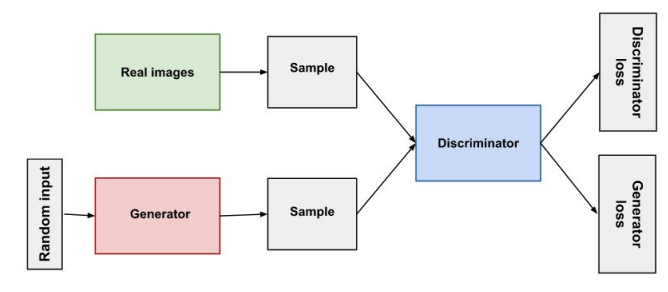
\includegraphics[width=0.99\linewidth]{img/GAN-Overview.png}
                        \caption{Esquema de funcionamiento de una GAN}
                    \end{minipage}
                    \begin{minipage}[h]{0.75\textwidth}
                        \centering
                        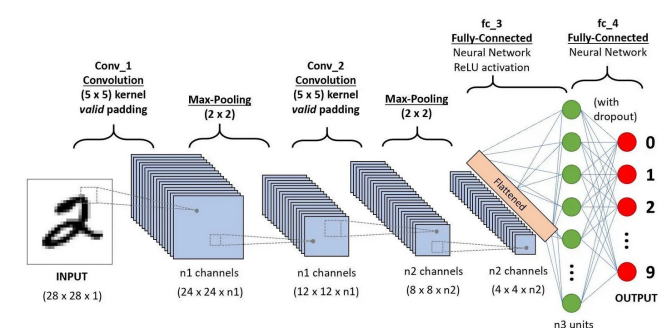
\includegraphics[width=0.99\linewidth]{img/CNN-Overview.png}
                        \caption{Esquema de funcionamiento de una CNN}
                    \end{minipage}
                \end{figure}
                
                \item \textbf{Basados en Búsqueda:} Muchos de estos métodos están basados en algoritmos evolutivos, los cuales están basados en IA que imitan el comportamiento de la evolución biológica \cite{CognizantEvolutionaryAlgorithm}. No obstante el uso de estos algoritmos evolutivos presentan problemas en la codifican el terreno en cromosomas, el diseño de la funciones de ajuste y la variación del terreno, lo que produce como resultado terrenos demasiado planos comparados con los reales. 
                \begin{figure}[h]
                    \centering
                    \includegraphics[width=0.65\textwidth]{img/Diagrama de relación entre PTG, SBPCG y EA.png}
                    \caption{Diagrama de relación entre los algoritmos generación procedural (PTG), basados en búsqueda (SBPCG) y evolución (EA)\cite{Raffe2012}}
                \end{figure}\newpage

                \item \textbf{Generación Procedural Inversa:} En estos métodos se extraen parámetros para generar terrenos a partir de ejemplos, para luego recrear las características del terreno de ejemplo usando los parámetros aprendidos de estos. Un caso de este método es el que se da en \cite{Emilien2015}, donde se propone aprender sobra la densidad de vegetación en un área, para a recrear una brocha que instancie vegetación usando esta densidad obtenida.
            \end{itemize}

        \subsubsection{Métodos basados en Bocetos}
        Estos métodos consisten en crear terrenos a partir de una información específica del usuario sobre la forma que este tendrá y sus características. Estos métodos mejoran el control sobre el terreno generado dando al usuario la habilidad de dar aspecto al terreno a través de interfaces como si se dibujaran. La desventaja de estos métodos es el menor realismo que logran en comparación con otros métodos.
            \begin{itemize}
                \item \textbf{Boceto 2D:} Este método consiste en generar trazas 2D que representan las siluetas de las montañas que se quieren hacer visibles desde el ángulo de la cámara. 
                \item \textbf{Boceto 3D:} En lugar de hacer bocetos 2D para pasarlo a 3D mediante reconstrucción, se trabaja directamente con vectores 3D desde el comienzo o curvas en algunos casos. Una vez las referencias 3D están colocadas se produce la voxelización de los vectores que los transforma en aproximaciones discretas dando así estructura al terreno.
            \end{itemize}

            \begin{figure}[h]
                \centering
                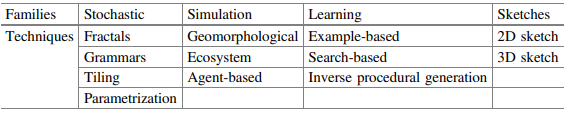
\includegraphics[width=0.8\textwidth]{img/terrain-generation-techniques.png}
                \caption{Clasificación general de las técnicas de generación según \cite{Valencia-Rosado2019}}
            \end{figure}
        
    % \subsection{Algoritmos para Reducción de Geometría: Estrategias para la Optimización de Geometría y LOD}

    %     \begin{enumerate}
    %         \item \textbf{Método de SubDivision Iterativo}
    %         Mapa de altura -> iterativo. Cada iteración introduce gran cantidad de aleatoriedad para generar mayor detalle de elevación. Manera de ajustar el comportamiento del algoritmo: ajustar el número de pasos de subdivisiones y desplazamiento inicial. Estos métodos no proporcionan ninguna manera de influir en las características, tales como montañas o valles. \cite{AnalisisAlgoritmosAmbientesVirtuales}

    %         Este método de Nicholas Rudzicz y Clark Verbrugge se basa exclusivamente en la subdivisión repetida de polígonos. Componente clave del algoritmo -> conjunto de polígonos de gran tamaño que contiene todos los polígonos con una superficie.
    %     \end{enumerate}


    \subsection{Generación de Poblaciones}

        La generación de ciudades, poblaciones o asentamientos conlleva la creación de edificios con organización siguiendo algún patrón y de caminos o carreteras. Para ello se han llevado a cabo diversas implementaciones de recreación de patrones de carreteras y generación de edificios pudiendo variar en en función del estilo arquitectónico. 

        Existe una gran diversidad de patrones que se pueden dar en la generación de carreteras (lo cual constituye un factor primordial en la generación de ciudades), y estos patrones son producto de numerosos factores. Las poblaciones pueden contener un gran número de patrones prevalecieres en distintas zonas, lo que las hace objetos anárquicos en cierta medida y por tanto difíciles de modelar. 

        En este apartado se hará una revisión de los modelos de generación de ciudades siguiendo el estudio realizado por George Kelly y Hugh McCabe en \cite{kelly2006survey}, donde se hace una evaluación de los resultados obtenidos por los distintos métodos en base al realismo, escala, variabilidad, entrada necesaria, eficiencia, control y aplicabilidad en tiempo real.

        Los modelos son los siguientes:

        \subsubsection{Diseño Grid y Primitivas Geométricas :} Este método presentado por Stefan Greuter en \cite{Greuter2002}\cite{Greuter2003} propone una solución para generación de ciudades en tiempo real, la cual se aplicó en una aplicación llamada \textit{Undiscovered City} donde se crea una red de carreteras usando un diseño de grid sobre un el cual se posicionan las construcciones generadas usando una combinación de primitivas geométricas. Las carreteras son creadas en base a un tamaño regular de los bloques que serán las parcelas donde se construirán lo edificios, el cual se puede ajustar de manera global. En cuanto a la generación de construcciones, se crea la geometría usando el concepto de combinación de primitivas geométricas para formar las secciones de los edificios.
        
            En cuanto a la evaluación de este modelo, los resultados producen patrones muy regulares de edificios dada su distribución en diseño de gird dando una apariencia muy homogénea, que sumado al aspecto que dan los edificios, los resultados se podrían considerar realistas pero no convincentes. En cuanto a escala, este sistema no parece tener limitación para la generación más allá de la limitación del tamaño de los números enteros para la generación de coordenadas de los bloques. A pesar de que la geometría para cada construcción es diferente, la cantidad de variación que se produce es insuficiente para emular ciudades reales. La aplicación mencionada que se realizó usando este método es standalone, por lo que no se necesitan datos de entrada. Aunque los tamaños de bloque se pueden ajustar, la generación no es interactiva y se realiza de manera automática. Por último, en cuanto a su aplicación en tiempo real, este sistema está diseñado par aplicaciones en tiempo real, por lo que se pueden renderizar grandes ciudades en hardware de equipos comunes a buenas tasas de refresco gracias a optimizaciones como el cacheado de geometría y el frustrum culling.
        
        \subsubsection{Sistemas L:} Yoav Parish y Pascal Muller en su artículo "Procedural Modeling of Cities" \cite{Parish2001} presentaron su aplicación, de la cual ya se habló en las herramientas existentes relacionadas con este trabajo, por lo que sigue estando vigente. La aplicación que presentaron es CityEngine, que consiste en un conjunto de componentes, incluyendo generación de carreteras, construcción de edificios y fachadas que se unen  para formar una pipeline para generación de ciudades. Los Sistemas L son la técnica clave en torno a la que gira la generación procedural de este modelo. 
        
            CityEngine usa una forma extendida de los Sistemas L llamados \textit{Auto-sensitivos-L} para construir redes de carreteras de manera que se tenga en cuenta el crecimiento existente para su generación. La generación de carreteras se lleva a cabo usando dos tipos de reglas: \textit{Objetivos Globales}, que definen los tipos de carreteras (principales y secundarias), su patrón geométrico y el criterio de elevación que han de seguir, y \textit{Restricciones Locales} las cuales determinan que las carreteras se creen en áreas legales en base a condiciones. 

            Las construcciones usando Sistemas L como el que se proponen se generan en diferentes fases: definir emplazamiento de las construcciones, crear la geometría de los edificios y generar la textura de las fachadas, usando diferentes Sistemas L que permiten generar diferentes tipos de edificios, los cuales son determinados por la zona del mapa.

            En la discusión de este modelo se determina que los Sistemas L proveen un método efectivo para la generación realista de paisajes urbanos con áreas verdes incluidas, a pesar de que las construcciones resultan ser un poco básicas. En cuanto a entradas de datos, se requiere como mínimo un mapa geográfico con información sobre elevación, vegetación y los límites acuáticos, por lo que el tamaño de este input es el principal factor que puede limitar el tamaño de las ciudades generadas. Se pueden generar un rango notable de redes de carreteras con distintos patrones y también variedad de edificios, aunque en un rango algo limitado. En cuanto al control, parece estar sujeto a la cantidad de imágenes de mapas que puedan ser pasados como datos de entrada. Aunque la generación es eficiente, pudiendo crear grandes redes de carreteras en menos de dies segundos, no permite la generación en tiempo real dado que no implementa técnicas de optimización como culling de geometría o LOD.
        
            \begin{figure}[h]
                \centering
                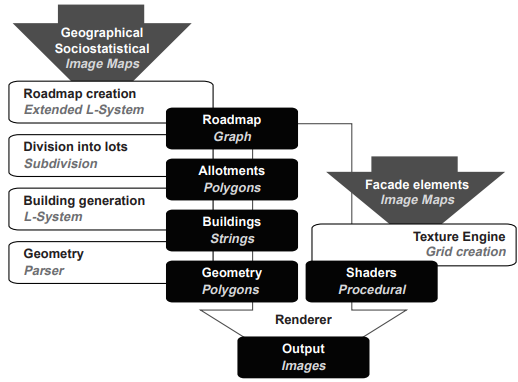
\includegraphics[width=0.7\textwidth]{img/cityengine-diagram.png}
                \caption{Diagrama de la estructura del algoritmo para CityEngine obtenido de \cite{Parish2001}}
            \end{figure}

        \subsubsection{Simulación basada en Agentes:} Este método nombrado anteriormente -al igual que los Sistemas L- en la generación procedural de terrenos también tiene aplicación para la generación de ciudades. En \cite{Watson2003} se presenta una solución llamada \textit{CityBuilder} que simula ciudades usando agentes como desarrolladores, autoridades planificadoras y constructores de carreteras. Además de simular la generación de la ciudad, este modelo también simula el crecimiento y desarrollo de la misma a lo largo del tiempo.

            Para la generación de carreteras se definen dos tipos de agentes: \textit{Extendedores}, los cuales buscan extender la red de carreteras acorde a la densidad de carreteras desde la que se parte, proximidad a intersecciones  y desviación del punto de salida. Y los \textit{Conectores}, quienes chequean la distancia para ir de un punto a otro dentro de un radio para crear nuevas redes en caso de que la distancia sea mayor de un umbral. Las carreteras son creadas acorde a un patrón de grid, aunque la desviación de este parámetro puede especificada mediante parámetros.

            En la generación de edificios se realiza la interacción de varios tipos de agentes, pero son principalmente los llamados \textit{Desarrolladores}, quienes cumplen el rol de desarrolladores urbanos obteniendo permisos de planificación, comprando y vendiendo parcelas de tierra. Existen distintos tipos de desarrolladores definidos: residenciales, comerciales e industriales. En este sistema se crean carreteras y se define el uso de las parcelas mediante la interacción de los agentes mencionados, lo que se usa para determinar el tipo de edificios que ocuparán las parcelas, pero no se generan ni geometría de edificios ni texturas.

            En la evaluación de ste método se puede decir que a pear de no producir construcciones los mapas generados parecen realistas, aunque la escala de estos es limitada, siendo similar a la de una villa o pueblo pequeño, pero no ciudades. Permite variedad de zonas, pudiendo ser estas residenciales, comerciales o industriales, y se necesitan mapas de altura del terrenos y el nivel del mar como entradas mínimas para determinar las áreas legales donde los edificios serán emplazados. Además incorpora una GUI que permite modificar parámetros de manera interactiva con un sistema de painting . Los aspectos negativos de este método son que es un algoritmo computacionalmente intensivo y consume mucho tiempo teniendo en cuenta la escala de los resultados que produce, además de que no hay si quiera consideraciones de ejecución de este método en tiempo real.
        
        \subsubsection{Generación basada en Plantillas:} Este es un método alternativo a los anteriores propuesto en el artículo \cite{Sun2002} donde la idea básica es generar un sistema donde una plantilla de red de carreteras es aplicada sobre un mapa geográfico como un plano y las carreteras son moldeadas siguiendo restricciones locales. 
        
            En este modelo la red de carreteras es representativa de la distribución de población, la cual viene dada por una plantilla basada en población implementada usando diagramas de Voronoi, donde los puntos de densidad poblacional son la entrada para generar dichos diagramas. Existen varias plantillas que sirven como patrones de crecimiento de la red de carreteras, que son las plantillas: \textit{Modo raster, Modo Radial y Modo Mixto}. Estas plantillas definen únicamente el patrón ideal de la red, pero estas se adaptan siguiendo restricciones locales que hacen que se eviten obstáculos como zonas de agua y de alta elevación. 

            Con este método se reflejan patrones encontrados en ciudades, pero no alcanzan la complejidad ni escala de las redes reales de ciudades. Aunque se pueden combinar patrones, solo se pueden combinar dos, lo que resulta insuficiente. Las plantillas de población y de crecimiento de carreteras y sus deformaciones ne base a las restricciones ofrecen variabilidad limitada. Al ser un método basado en plantillas requiere varias entradas, como mapas de alturas, geográficos y de densidad de población.

            El método no ofrece control dado que se basa en información estática y no hay interacción con el usuario. No hay información sobre la eficiencia del método y por tanto tampoco sobre su aplicación en tiempo real.
        
            \begin{figure}[h]
                \centering
                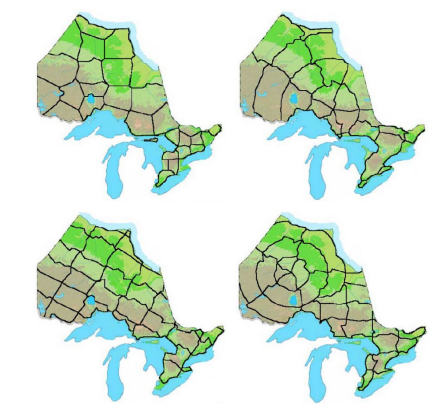
\includegraphics[width=0.5\textwidth]{img/template-terrains.png}
                \caption{Plantilla basada en población (arriba izq.), Modo Radial (arriba der.), Modo Raster (abajo izq.), Modo Mixto (abajo der.).}
            \end{figure}

        \subsubsection{Gramáticas de separación:} El método que se discute a continuación es el presentado en \cite{Wonka2003}, donde se propone la generación realista de edificaciones a través de un tipo de gramática llamada \textit{gramática de separación}, las cuales están basadas en el concepto de forma. Aunque este es un método de generación de construcciones, no de ciudades, y dado que este TFM va a ser desarrollado en Unity, que es un motor de videojuegos, no de modelado, no tiene aplicación. No obstante, es una técnica empleada en la generación de ciudades a nivel general y se ha creído conveniente nombrarla como parte del estado del arte de este campo, aunque no se analizará tan en profundad como los anteriores métodos.
        
            Este método genera construcciones usando objetos llamados \textit{formas básicas}, las cuales son parametrizadas, etiquetadas y dotadas de atributos simples. Se parte de un estado inicial y se realizan transformaciones en un proceso iterativo usando reglas de una base de datos, las cuales separan las construcciones en fachadas, las fachadas en secciones estructurales y estas secciones en componentes como ventanas y demás. Los atributos de las formas desde las que se parte son propagados a los componentes y gramáticas de control pueden cambiar las propiedades de las formas básicas para aplicar diferentes conceptos de diseño espacial. 

            Este método produce edificios muy realistas y con gran variedad que incluso permite recrear estilos arquitectónicos. El numero de edificios generables con este sistema es limitado y no llega a la escala de una ciudad. Se requiere una entrada significativa -una base de datos con reglas y atributos que modelen los edificios. El algoritmo, a pesar de ser complejo es eficiente permitiendo incluso la exploración en tiempo real, no obstante el número de edificios mostrables al mismo tiempo es limitado. También ofrece control a través de la modificación de las reglas directamente de la base de datos.

        \subsubsection{Generación Procedural de Poblados en Tres Pasos:} Emilien en su artículo "Procedural Generation of Small Cities in Three Steps" \cite{Emilien2012} propone un método para generar villas o pueblo pequeños de tres pasos que recrea los pequeños asentamientos europeos que utilizan las características del terreno. El método consta de tres pasos: el primero es un proceso iterativo basado en mapas de interés para generar semillas de asentamiento y los caminos que los conectan, teniendo en cuenta el hecho de que un nuevo camino atrae a nuevos asentamientos y nuevos asentamientos conduce a una extensión de los caminos. El segundo paso es un método de conquista anisotrópico que segmenta la tierra en parcelas alrededor de las semillas de asentamiento. Finalmente se introduce una \textit{gramática de forma abierta (open shape grammar)} para generar geometría 3D que se adapte a la pendiente local y terreno local. Esto se consigue creando primero los pisos y el techo y después añadiendo elementos de la fachada. Las \textit{Open Shape Grammars} incorporan mecanismos de adaptación mediante restricciones como la no colisión con el suelo, alienación de elementos y demás reglas. 
        
            Este método permite crear de manera poblados con formas realistas comparadas con las de las formas de las villas reales, con un número de vecinos y de esquinas similares, además de una generación realista de edificios gracias al método basado en \textit{Open Shape Grammars}. Solo requiere la información del terreno como mapa de alturas y cuerpo de agua como entrada para la generación y permite el control a través del suo de mapas de interés para crear las semillas de asentamiento y las reglas para generación de construcciones. La escala de los resultados no excede el tamaño de pequeñas villas como se indica en su objetivo y no hay datos del rendimiento, por lo que no se puede evaluar correctamente su uso en aplicaciones de tiempo real.
        
            \begin{figure}[h]
                \centering
                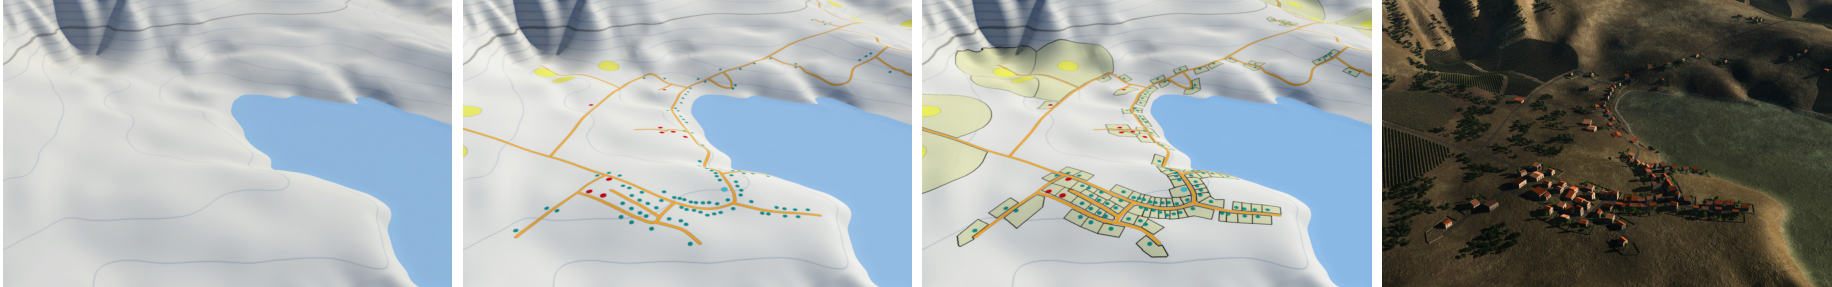
\includegraphics[width=1\textwidth]{img/procedural-generation-of-villages-on-arbitrary-terrains-overview.png}
                \caption{Muestra del funcionamiento del método: dado un terreno se genera el esqueleto del poblado (caminos and semillas de asentamiento), después se añaden las parcelas y finalmente las geometrías de las casas.}
            \end{figure}   
        % \subsubsection{Algoritmo de Distribución de Poblaciones basado en Modelos de Asentamiento:} Investigación académica sobre modelado de asentamientos.

        %     \begin{itemize}
        %         \item \textbf{Generación procedural de aldeas utilizando un sistema basado en nodos.} Disponible en PDF.
        %         \item \textbf{Generador procedural de terrenos para Unity - Universidad de Jaén.} Disponible en PDF.
        %     \end{itemize}

        % \subsection{Técnicas de Simulación de Entornos Naturales}
        % \begin{itemize}
        %     \item \textbf{Métodos para Simular Biomas y Ecosistemas: }
        %     \item \textbf{Métodos para Simular Climas y Fenómenos Atmosféricos: }
        %     \item \textbf{Métodos para Modelar Masas de Agua y su Interacción con el Terreno: }
        % \end{itemize}

        \subsection{Métodos Complementarios}
        En este apartado se discutirá sobre métodos que ayudan en la generación de los elementos troncales de este trabajo pero que no son temas principales. Aún así estas técnicas pueden jugar un papel crucial en el realismo y coherencia visual, por lo que son de importante relevancia y su rendimiento también juega un papel clave, ya que pueden  procesos fundamentales como la instanciación de objetos y la corrección de bordes
            \subsubsection{Métodos para Simplificar la Geometría: }
            Dado que se deberá optimizar el rendimiento lo máximo posible, la reducción de geometría es un paso indispensable debido al ahorro en cálculo que supone. Existen varios métodos para simplificar la geometría de los objetos de una escena:
                \begin{itemize}
                    \item \textbf{Colapso de bordes: }El colapso de bordes implica la fusión de vértices adyacentes, lo que reduce el número de bordes en la malla. Este método es preferible en modelos geométricos \cite{linkedinmeshsimplification}. 
                    \item \textbf{Colapso de aristas: } El colapso de arista es un método similar al anterior, pero en este caso se elimina una arista  manteniendo la cantidad de vértices. Este método es preferible en modelos orgánicos  \cite{linkedinmeshsimplification}.
                    \item \textbf{Agrupación en clústeres de vértices: }La agrupación en clústeres de vértices divide la malla en celdas y reemplaza cada celda con un vértice central o promedio, lo que simplifica la estructura \cite{linkedinmeshsimplification}. Rossignac y Borrel proponen un método en \cite{Rossignac1993} que consiste en colocar una caja delimitadora alrededor del modelo original y dividirla en una cuadrícula, agrupando los vértices que caigan dentro de la misma celda y actualizando las caras del modelo. Aunque es un método efectivo para la simplificación, la calidad de los resultados parece ser baja y no tampoco permite un gran control sobre la cantidad de cara resultantes.
                    \item \textbf{Simplificación basada en curvatura: }Este método utiliza la curvatura de la superficie para identificar y conservar las características importantes de la geometría, permitiendo así realizar simplificaciones conservando la mayor fidelidad y las características de la original. En \cite{Jinete2015} se describe un método para el remallado de rostros humanos que se basa en alinear los bordes de la superficie de la malla utilizando análisis del tensor de curvatura de esta para ajustarla de manera anisotrópica. Uno de los algoritmos que corresponde con este tipo de métodos es el algoritmo de Ramer-Douglas-Peucker (RDP) para reducir el número de puntos utilizados en la aproximación de una curva. La forma inicial del algoritmo fue propuesta independientemente en 1972 por Urs Ramer, en 1973 por David Douglas y Thomas Peucker, y algunos más en la siguiente década. Este algoritmo también es conocido con el nombre de algoritmo de Douglas-Peucker \cite{RamerDouglasPeucker}.                
                    \item \textbf{Decimación de vértices: }Estos métodos es otro método de reducción de vértices y aristas de la malla. En el método presentado en \cite{Schroeder1992} se describe un algoritmo que selecciona de manera iterativa un vértice para eliminar, elimina todas las caras adyacentes y vuelve a triangular el agujero resultante.
                    \item \textbf{Métrica de error cuadrático: }La métrica de error cuadrático es el método que se utiliza para minimizar la desviación entre la malla simplificada y la original, colapsando aristas o vértices teniendo en cuenta la orientación de la cara usando \cite{linkedinmeshsimplification}.
                \end{itemize}

            En este subapartado cabe mencionar los trabajos de Jain, Aryamaan y Sharma en su artículo "Learning Based Infinite Terrain Generation with Level of Detailing" \cite{Jain2022} donde proponen un framework generativo basado en aprendizaje para generar terrains infinitos, con un enfoque novedoso también basado en aprendizaje para terrenos con nivel de detalle, el cual integra un método de renderizado basado en quadtrees y completado de detalles con imágenes para terrenos con super resolución.
            \begin{figure}[h]
                \centering
                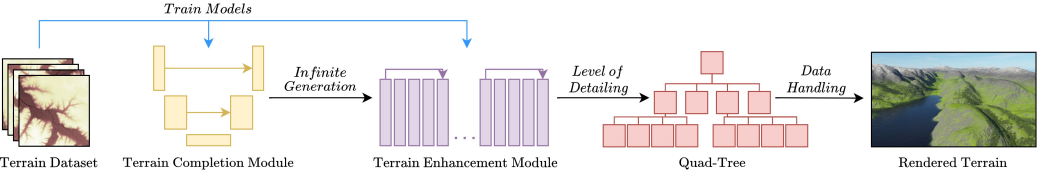
\includegraphics[width=0.9\textwidth]{img/framework-overview.png}
                \caption{Descripción general del framework presentado en "Learning Based Infinite Terrain Generation with Level of Detailing"\cite{Jain2022}}
            \end{figure}

            También el de Jian Wu, Yuanfeng Yang, Shengrong Gong y Zhiming Cui en su artículo "A New Quadtree-based Terrain LOD Algorithm" \cite{Wu2010ANQ}, donde se expone un nuevo algoritmo de LOD de terreno que utiliza un quadtree, el cual puede satisfacer la necesidad de renderizado en tiempo real para datos de terreno masivos, y un nuevo algoritmo de eliminación de grietas.
            
            \subsubsection{Modelos de Distribución de Objetos: }
                \begin{itemize}
                    \item \textbf{Basados en Puntos de Interés: }Estos modelos toman puntos concretos y centran la mayor distribución de objetos entorno a ellos. Estos puntos de interés pueden ser determinados por mapas sirviendo de entrada para el sistema de distribución. También se pueden determinar los puntos en base a ciertos criterios o características del entorno donde se distribuyan. En \cite{Parish2001} se hace uso de mapas de distribución de población extrayendo de estos los puntos para generar diagramas de Voronoi con los que se producirá la generación de edificios.
                    \item \textbf{Basados en Probabilística: }Una de las maneras más comunes de hacer distribuciones de objetos es siguiendo distribuciones probabilísticas. La distribución uniforme o la de Poisson son las más utilizadas. Existen diversos artículos como \cite{autobiomes}, \cite{landmasses-terrain} o \cite{GaschGarcia2021} donde se emplea el muestreo basado en alguna de estas distribuciones para la instanciación de activos en generación procedural. En los artículos mencionados se usa concretamente el muestre de disco de Poisson, donde se busca que haya la mayor distancia posible entre un par de objetos evitando agrupaciones pero produciendo una distribución menos regular que la uniforme. El término "disco" se refiere a las formas que se utilizan para definir la separación mínima entre los objetos.
                    \item \textbf{Basados en Gramáticas o Reglas: }De nuevo, esta técnica vuelve a aparecer, esta vez como modelo de distribución. En \cite{autobiomes} se combina la distribución de disco de Poisson, con el uso de reglas para modelar qué especies deben aparecer más frecuentemente o más cerca unas de otras. 
                    \item \textbf{Basados en Análisis de Terreno: }Algunos sistemas utilizan permiten distribuir objetos de acuerdo a las características topográficas del terreno. Por ejemplo en el paper "Procedural Generation of Villages on Arbitrary Terrains" \cite{Emilien2012}, los objetos son distribuidos de acuerdo a las características del terreno.
                \end{itemize}

            \subsubsection{Métodos de Texturizado: }
            En generación procedural es importante tener en cuenta el realismo del terreno generado (en caso de que se pretenda realismo) no solo en base a la estructura y topografía del terreno generado, sino en los colores y aspecto que presenta. Para ello, las técnicas de texturización son una parte importante a tener en cuenta. Aquí se presentan algunas técnicas habitualmente utilizadas \cite{texturing2024}.
                \begin{itemize}
                    \item \textbf{Procedural: }Para crear texturas mediante programación utilizando algoritmos y funciones matemáticas. Esta técnica se utiliza a menudo para crear patrones complejos y texturas naturales como nubes, rocas o agua.
                    \item \textbf{Basada en Imágenes: } Consiste en aplicar imágenes en modelos 3D para crear detalles de superficie realistas.
                    \item \textbf{Pintura : } El uso de software de pintura digital se puede utilizar para crear texturas estilizadas o artísticas. 
                    \item \textbf{Stenciling: } Al aplicar texturas selectivamente a áreas específicas de un modelo 3D usando máscaras.
                    \item \textbf{Mezclado de Texturas: }Para combinar múltiples texturas para crear detalles de superficie complejos como óxido o suciedad. Dentro de esta categoría podríamos encuadrar los \textbf{shaders triplanares}, los cuales permiten combinar varias texturas con transiciones suaves entre ellas, y son ampliamente utilizados para generación procedural. 
                    \item \textbf{Mapeo de Normales: }Simula la apariencia de golpes, abolladuras o cualquier otro tipo de detalle en una superficie plana mediante el uso de una imagen 2D que codifica las normales de superficie.
                    \item \textbf{Mapeo de Desplazamiento: }Consiste en agregar detalles geométricos a la superficie de un modelo 3D mediante el uso de una imagen en escala de grises para deformar la geometría de la superficie.
                    \item \textbf{Tiling: }Compone texturas de patrones que se pueden repetir sin problemas en una superficie grande como un suelo o una pared.
                \end{itemize}


        \subsection{Optimización y Rendimiento}
            
            \subsubsection{Técnicas y Algoritmos de Optimización}
                Dado que la herramienta que se pretende desarrollar debe funcionar en tiempo real, es conveniente implementar técnicas que permitan ahorrar el mayor tiempo de computación y memoria posible con el fin de obtener un rendimiento óptimo. A continuación se presentan varias técnicas ampliamente utilizas para la optimización de código.
                \begin{itemize}
                    \item \textbf{Culling:} El culling es una técnica ampliamente utilizada en gráficos que consiste en ocultar elementos no visibles en la escena para optimizar la carga de trabajo reduciendo el número de polígonos que procesar. Existen diversos tipos de culling como el \textit{Frustum Culling}, el cual omite todos aquellos objetos que queden fuera del \textit{frustum}, el cual representa el espacio 3D de visión de la cámara, el \textit{Occlusion Culling} que omite aquellos objetos o polígonos que se encuentran no visibles a la cámara aunque sí estén dentro del espacio de visión de esta y otros tipos de culling como el \textit{Camera Culling} que se asocia más con propiedades de la cámara como su ángulo, distancia a esta, etc, más que con el capo de visión.
                    \item \textbf{Nivel de detalle:} El nivel de detalle o LOD, es otra técnica de optimización que se utiliza a menudo en gráficos para reducir la complejidad de la geometría de una escena en función de la distancia a al cámara. A mayor distancia a la cámara, menor número de polígonos y por tanto, menor definición tendrán los objetos que implementen esta técnica. Los objetos podrán tener de esta manera diferentes geometrías, cada una de ellas asociada a un LOD distinto que se mostrará en base a la distancia a la cámara.
                    \item \textbf{Chunking:} Chunking es una técnica que permite la generación de geometría por lotes en lugar de tener que crearla de una vez. Esta técnica es ampliamente utilizada en generación de terreno procedural, por lo que atañe directamente al tema de este proyecto, y es utilizada ampliamente en juegos como Minecraft para la generación de sus mundos. Con esta técnica se lleva a cabo la carga y descarga dinámica de estos lotes la cual se puede combinar a su vez con otras técnicas de optimización como el LOD, aunque también puede conllevar otras implicaciones que añaden cierta carga computacional como el ajuste de los bordes entre los distintos chunks en algunos casos.
                    \item \textbf{Instanciación con GPU:} La creación de instancias con GPU es un método de optimización que genera múltiples copias de una mesh con el mismo material en una única llamada de dibujo. Es útil para dibujar cosas que aparecen varias veces en una escena, por ejemplo, árboles o arbustos.                 
                    La creación de instancias con GPU genera mallas idénticas. Para agregar variación y reducir la apariencia de repetición, cada instancia puede tener diferentes propiedades, como Color o Escala. Esta técnica es compatible con el sistema de Iluminación Global Baked de Unity y con los shaders estándar de Unity. Al utilizar instanciación en GPU, se mejora significativamente el rendimiento al reducir la carga de la CPU y optimizar la renderización de elementos repetitivos en la escena. \cite{unityGPUInstancing}
                    \item \textbf{Paralelización:} Consiste en realizar la ejecución del código en distintos hilos aprovechando el máximo rendimiento de la CPU al hacer que trabajen todos los núcleos sin saturar el hilo principal. En Unity existe el JobSystem, del cual hablaremos más tarde para la paralelización y ejecución de código paralelo de manera segura. Además de JobSystem también cabe mencionar las corrutinas, la cuales permiten ejecutar código en distintos hilos de manera asíncrona, no interrumpiendo la ejecución del hilo principal.
                    \item \textbf{Diseño en capas:} Hacer un diseño de la lógica en capas puede ayudar a reducir la complejidad y mejorar la mantenibilidad y escalabilidad del código. En Unity esto puede llevarse a cabo mediante el uso de prefabs, los cuales pueden derivar unos de otros, heredando la lógica asociada a ellos. 
                    \item \textbf{Profiling:} El uso de herramientas de manera metódica que permitan la detección de cuellos de botella, puntos de ajuste o de optimización también es crucial para poder obtener un rendimiento óptimo. En Unity existen diversas herramientas que permiten el ajuste de las partes que afecten o ralenticen la ejecución:
                    \begin{itemize}
                        \item \textbf{Profiler:} Esta herramienta está integrada en el propio editor de Unity y provee información valiosa acerca del rendimiento de los componentes que intervienen en la ejecución en CPU. Se usa para hacer diagnósticos de los problemas de rendimiento y optimización.
                        \item \textbf{Graphics Debugger:} Esta herramienta depura la aplicación y permite analizar el rendimiento en la GPU para detectar posibles problemas en el renderizado o los shaders.
                        \item \textbf{Unity Remote:} Con esta herramienta se pueden probar y depurar las aplicaciones directamente en dispositivos para optimizar el rendimiento en dispositivos como móviles o tablets, inclusive gafas de RV.
                    \end{itemize}
                \end{itemize}
           
        \subsection{Optimizaciones para la Compatibilidad con Realidad Virtual}

            Para el desarrollo en Realidad Virtual, hay ciertas consideraciones adicionales que se deben tener en cuanta para una experiencia óptima en términos de rendimiento e inmersividad. A continuación se detallan algunas de ellas.
            
            \subsubsection{Optmizaciones de Rendimeinto Específicas}
            Ya se han nombrado varias técnicas para la mejora del rendimiento, aún así, caben destacar algunas más específicas especialmente importante ciado se trata de aplicaciones en RV. \cite{fastercapital} \cite{linkedinoptimization}

            \begin{itemize}
                \item \textbf{Optimización de assets:} Dado que en realidad virtual se requiere de una renderización doble de la escena para cada visor, las escenas deben tener una cantidad de polígonos muy cuidado, y texturas optimizadas, de lo contrario se verá afectado el frame rate. 
                \item \textbf{Minimización de efectos de post-procesado:} De nuevo, la doble renderización es la causante de la necesidad de minimizar los efectos de post-procesado. Debido a la alta carga de trabajo que ya presenta esta tarea para la tarjeta gráfica, los efectos aumentarían dicha carga pudiendo ralentizar la tasa de refresco.
                \item \textbf{Tipos de iluminación:} Las luces estáticas y Mapas de Luces para proyectos de RV son la opción preferible debido a que es la opción de iluminación más económica de renderizar. Si se necesita usar iluminación dinámica, se debe limitar la cantidad de luces dinámicas a lo mínimo posible. Esta técnica es utilizable para cualquier tipo de aplicación, al igual que las anteriores descritas, pero en RV cobran especial importancia dado su impacto en el rendimiento.
                \item \textbf{Efectos visuales (VFX):} Algunos trucos de VFX, como usar Texturas SubUV para simular fuego o humo, no se mantienen muy bien cuando se ven en RV. En muchos casos, se necesitará usar mallas estáticas en lugar de partículas 2D para simular efectos como explosiones o estelas de humo. Los efectos de campo cercano, o efectos que ocurren muy cerca de la cámara, funcionan bien en RV, pero solo cuando están compuestos de partículas de meshes estáticas.
                \item \textbf{Evitar la transparencia:} En gráficos 3D, renderizar la transparencia es extremadamente costoso, porque la transparencia generalmente debe reevaluarse por frame para asegurarse de que nada haya cambiado. Debido a esta reevaluación, renderizar la transparencia en RV puede ser tan costoso que su costo supera sus beneficios.

            \end{itemize}

            \subsubsection{Estrategias para mejorar la Inmersividad}
            \begin{itemize}
                \item \textbf{Mecánicas de locomoción adecuadas:}  Elegir mecánicas que sean cómodas e intuitivas para el usuario, considerando las experiencias físicas de la RV. 
                \item \textbf{Escala del entorno:} Mantener la consistencia en las métricas de los elementos del entorno es fundamental para tener una experiencia inmersiva, ya que los usuarios de RV perciben la escala con más precisión que en entornos de pantalla plana.
                \item \textbf{Uso de audio:} Con sonido ambiental adecuado se puede mejorar la experiencia inmersiva mejorando la sensación de presencia en el entorno que se genere.
                \item \textbf{Limitar el mareo por movimiento:} El mareo por movimiento que puede afectar a los usuarios durante experiencias inmersivas. La siguiente lista describe algunas buenas prácticas para limitar el malestar que los usuarios pueden experimentar en la realidad virtual:
                \begin{itemize}
                    \item \textit{Mantener la frecuencia de refresco:} Los bajos fps pueden causar mareos, por lo que es fundamental conseguir un buen frame rate.

                    \item \textit{Mantener a los usuarios en control de la cámara:} Las cámaras cinematográficas, o cualquier cosa que tome el control de los movimientos de la cámara lejos del jugador, contribuyen al malestar del usuario en experiencias inmersivas. Se deben evitar efectos de cámara, como el movimiento de la cabeza y el temblor de la cámara, ya que pueden provocar malestar si el usuario no los está controlando.
                    
                    \item \textit{El FOV debe coincidir con el dispositivo:} El valor del FOV (field of view o campo de visión) se establece a través del SDK del dispositivo y la configuración interna, y coincide con la geometría física del casco y las lentes. Por esta razón, el FOV no debe ser modificable por el usuario. Si se cambia el valor del FOV, el mundo puede parecer distorsionado al girar la cabeza, lo que puede provocar mareo.
                    
                    \item \textit{Luces y colores más tenues, y evitar el desenfoque:} Al diseñar elementos para RV, es posible que necesites usar luces y colores más tenues de lo normal. La iluminación fuerte y vibrante en RV puede provocar desorientaciones. El uso de tonos más fríos y luces más tenues puede ayudar a prevenir el malestar del usuario. Esto también ayuda a prevenir el desenfoque entre áreas brillantes y oscuras en la pantalla.
                    
                    \item \textit{La velocidad de movimiento no debe cambiar:} Los usuarios deben comenzar a toda velocidad en lugar de acelerar gradualmente hasta la velocidad máxima.
                    
                    \item \textit{Evitar los efectos de post-procesado que afecten significativamente lo que ve el usuario:} Evita los efectos posteriores como la Profundidad de Campo y el Motion Blur para prevenir el malestar del usuario.
                \end{itemize}
            \end{itemize}


            \subsubsection{Limitaciones Debido a la Realidad Virtual}
            Dada las características de la realidad virtual, se deben tener en cuenta ciertas técnicas que podrían no ser efectivas ni tener los resultados esperados cuando se utilizan en un dispositivo para RV. Aquí se presentan algunas limitaciones: \cite{unrealengineVR}

            \begin{itemize}
                \item \textbf{Iluminación global en espacio de pantalla:} Las técnicas en espacio de pantalla pueden generar diferencias entre las pantallas para los dos ojos en el HMD. Estas diferencias pueden causar molestias al usuario. Además de esto, la iluminación por píxel puede producir algunos artefactos que serán más evidentes en RV y también puede no tener en cuenta correctamente la profundidad de los elementos a la hora de iluminar, lo que puede dar una sensación menos inmersiva.
                \item \textbf{Ray Tracing:} Las aplicaciones de RV que utilizan trazado de rayos actualmente no pueden mantener la resolución y los fps necesarios para una experiencia de RV cómoda.
                \item \textbf{Interfaz de usuario 2D o Sprites tipo Billboard:} La interfaz de usuario 2D o los sprites tipo billboard no son compatibles con el renderizado estéreo ya que no se ven bien.
                \item \textbf{Mapeo de normales:} Cuando se ven mapas de normales en objetos en RV no tienen el mismo efecto dado que el mapeo normal no tiene en cuenta tener una pantalla binocular o paralaje de movimiento. Como resultado, los mapas normales a menudo se ven planos cuando se ven con un dispositivo RV. Es más conveniente usar mapas de paralaje en su lugar, aunque son específicamente recomendables para usar en caminos empedrados o superficies con detalles finos.
            \end{itemize}

            
            \subsubsection{DOTS Unity}
            En esta apartado se hablará sobre el el sistema DOTS de Unity compuesto por el Job System junto con el Burst Compiler y ECS (Entity Component System). Se comentarán los tipos de Jobs que hay y se analizará cuáles pueden ser los más propicios para la generación procedural. 

            \begin{itemize}
                \item \textbf{JobSystem: }El JobSystem, es un sistema que permite crear código multihilo de manera segura aprovechando todos los núcleos, haciendo que mejore el rendimiento de manera considerable. A continuación se describen los tipos de Jobs que existen \cite{unity-job-system}:
                \begin{itemize}
                    \item \textbf{IJob: }Ejecuta una única tarea en un hilo, en un job thread. Se utiliza este tipo de Job cuando no se necesita ejecución en paralelo.
                    \item \textbf{IJobParallelFor: }Ejecuta una tarea en paralelo. Cada job thread que se ejecuta en paralelo tiene un índice exclusivo para acceder de forma segura a los datos compartidos entre job threads. Es útil por cuando se pretende ejecutar una tarea en paralelo a un conjunto de datos, como por ejemplo, aplicar la misma operación a múltiples elementos.
                    \item \textbf{IJobParallelForTransform: }Ejecuta una tarea en paralelo. Cada job thread que se ejecuta en paralelo tiene un nodo transform exclusivo de la jerarquía de transformaciones en el que operar. Este job es útil cuando se necesita, por ejemplo, actualizar la posición de varios objetos en paralelo.
                    \item \textbf{IJobFor: }Igual que IJobParallelFor, pero permite programar el job para que no se ejecute en paralelo.
                \end{itemize}

                \item \textbf{Burst Compiler: } El burst compiler es un compilador de Unity que traduce el código IL/.NET bytecode a código nativo altamente optimizado usando LLVM. Se puede utilizar como un paquete de unity e integrarlo a través del Package Manager como cualquier otro paquete.\cite{UnityBurst}

                \item \textbf{ECS:} ECS para Unity (Entity Component System) es un marco orientado a datos compatible con GameObjects. Se podría considerar como un nuevo paradigma de programación orientado a datos que consta de tres partes principales: \cite{UnityECS}
                
                \begin{itemize}
                    \item \textbf{Entidades:} las entidades o cosas que pueblan el programa.
                    \item \textbf{Componentes:} los datos asociados con sus entidades, pero organizados por los datos en sí y no por entidad. 
                    \item \textbf{Sistemas:} la lógica que transforma los datos del componente de su estado actual a su siguiente estado.
                \end{itemize}
            \end{itemize}
        
            
            El JobSystem de Unity se puede combinar con el ECS y el Burst Compiler haciendo que el ECS reduzca el tiempo de cálculo de cada subproceso organizando los datos de manera más compatible con la caché y que el Burst optimice el código para reducir aún más el tiempo de trabajo, lo que permite aumentar el rendimiento enormemente. \cite {unityblog}
           

\section{Análisis de la investigación}
    \subsection{Aspectos Clave Abordados en el Estado del Arte}
    En el estado del arte se ha realizado principalmente el estudio y análisis de las herramientas previas y antecedentes con fines similares los que se pretenden llevar a cabo en este TFM. Se han estudiado softwares de Unity e independientes, incluso con compatibilidad con otros motores que realizan generación de terrenos de manera procedural con simulación de biomas e incluso de fenómenos atmosféricos con un alto grado de realismo, junto con softwares para la generación de poblaciones y asentamientos.
    
    Tras el estudio de los antecedentes se hizo una revisión de las técnicas más utilizadas y novedosas empleadas para la generación de terreno procedural en base a diversos estudios, artículos y sitios web. 
    
    Desde la generación de los propios terrenos con diversos métodos a las técnicas de optimización que se pueden llevar a cabo para mejorar el rendimiento de las aplicación que los implementen (incluido el sistema DOTS de Unity, del cual se hará uso en esta propuesta) y otros métodos complementarios involucrados en las técnicas y métodos más generales, pero necesarios para obtener buenos resultados. 
    
    En este estado del arte también se ha estudiado los distintos métodos para generación de ciudades y poblaciones, así como los aspectos relacionados con la compatibilidad con la realidad virtual, sus limitaciones y factores a tener en cuenta relacionados con las generaciones que se pretenden llevar a cabo.
    
    \subsection{Conclusiones}
    Del estudio realizado se pueden sacar diversas conclusiones. Comenzando por los métodos de generación de terreno, se han estudiado diferentes tipos, pero solo algunos son opciones reales para esta propuesta dadas las limitaciones derivadas de ser en tiempo real y compatible con realidad virtual. Las técnicas que se podrán tener más en cuenta son aquellas que permiten la generación paralela. 
    
    Los métodos basados en simulación para generar mapas de alturas tienen un coste computacional demasiado elevado en la mayoría de los casos para permitir una buena compatibilidad con la generación en tiempo real y la RV. Los métodos basados en aprendizaje requerirían de un entrenamiento previo de las IAs que trabajarían para generar el terreno, y otros algoritmos como el Wave Function Collapse no dan un resultado tan realista como otros métodos. En el caso de los generados por bocetos, los resultados que producen no se ajustan a los resultados buscados en esta propuesta y la metodología que siguen presenta dificultades para implementarla de manera paralela. Los métodos estocásticos son la propuesta más valorarle para ser implementada dado su bajo coste computacional y su fácil paralelización. En concreto, los métodos fractales son una solución ampliamente utilizada, siendo la opción elegida en la mayoría de métodos estudiados para la generación del terreno. 

    Tanto los métodos fractales basado en ruido como en los algoritmos recursivos de diamante-cuadrado o desplazamiento del punto medio son opciones válidas siendo muy habituales en los softwares y papers estudiados anteriormente, como se ha mencionado ya. En cuanto a la generación de biomas, se ha discutido sobre el coste de los algoritmos de simulación en tiempo real, no obstante, el paper ``AutoBiomes: procedural generation of multi-biome landscapes''\cite{autobiomes}, el cual se ha mencionado en el estado del arte en varias ocasiones, presenta un método apto para la generación en tiempo real, empleando tenencias de simulación en una versión simplificada abaratando su coste. Aunque el método que proponen está pensado para ser utilizado en tiempo real, que da por ver si será compatible con RV y se podrá ofrecer un buen rendimiento. Aun así, este paper ofrece un enfoque similar al que se pretende llevar a cabo en este trabajo, por lo que se tomará muy en cuenta su modelo para servir como base del que se desarrolle finalmente y se tendrán muy en cuenta las tenencias utilizadas dado que ya es una solución probada con fines parecidos y resultados satisfactorios para sus desarrolladores.

    Para la generación de poblaciones, se han estudiado varios métodos y sólo un par parecen ser los más válidos para esta propuesta. El método basado en diseño de grid y primitivas geométricas es una opción compatible con generación en tiempo real, aunque los resultados que ofrece parecen ser demasiado regulares, no obstante, estos aunque no son convincentes, permiten generar ciudades de manera realista, pero presenta el inconveniente de que conlleva el modelado de edificios, y Unity no permite el modelo de geometría. El método basado en tres pasos es un modelo que también es compatible con la ejecución en tiempo real, pero de nuevo presenta el problema del modelado, por lo que se deberá buscar una alternativa para la generación de construcciones que sea compatible con las capacidades de Unity. 

    Se ha hablado de métodos complementarios para la simplificación de geometría, distribución de objetos y texturizado. Todos estos procesos se deberían llevar a cabo cuando se implementen los métodos de generación principales del terreno, biomas y poblaciones. De los métodos de simplificación de geometría el método que más se ajusta dada las limitaciones para tratar con geometría es la decimación de vértices, donde se deberá llevar a cabo una omisión de ciertos vértices sin modificar la geometría. En cuanto a la distribución de objetos, todas las técnicas son candidatas y se pueden combinar, aunque como se ha dicho antes, las técnicas empleadas en Autobiomes pueden tener cierta preferencia, que en este caso se trataría de la distribución de disco de Poisson. Para la texturización, se contemplan el uso de texturas generadas proceduralmente y el mezclado de varias texturas, mediante shaders triplanares, dado que como se mencionó, es una técnica ya empleada en generación de terrenos procedurales.
    
    Por último se ha hablado de diversas técnicas de optimización y de factores clave a tener en cuenta para RV. En este aspecto se tratarán de implementar el mayor número posible de estas para mejorar el rendimiento al máximo. Técnicas como el culling, LOD, paralelización o chunking deberán ser puestas en práctica de manera obligatoria, dado que como se vio en las limitaciones provocadas por la compatibilidad con RV, una de las causas de mareo es debido a bajas tasas de refresco, por lo que la optimización queda en un total primer plano. Otras de las limitaciones de la RV como es la doble renderización y la sobrecarga en la GPU que producen los efectos de post-procesado debido a este factor, es un motivate para dejar fuera del proyecto recreación de fenómenos atmosféricos y otro tipo de recursos que hagan uso de la tarjeta gráfica y puedan ocasionar latencias. 

